\documentclass[12pt]{article}

% Package Imports
\usepackage{amsmath,amssymb}  % Math symbols
\usepackage{graphicx}         % For figures
\usepackage[margin=1in]{geometry}  % Standard margin
\usepackage{setspace}         % Adjust line spacing
\usepackage{authblk}          % For authors and affiliations
\usepackage{caption}          % For figure captions
\usepackage{subfigure} 
\usepackage{url}              % For clickable/line-breaking URLs
\usepackage[numbers, sort]{natbib} % 

% Title and Author Setup
\title{quantms-rescoring and multi-engine searching enable deep proteome coverage across quantitative proteomics, immunopeptidomics, and phosphoproteomics}
\author[1,2]{Chengxin Dai}
\author[3,4]{Ralf Gabriels}
\author[3,4]{Robbin Bouwmeester}
\author[5,6,7,8]{Jonas Scheid}
\author[9]{Henry Webel}
\author[3,4,10,11]{Lennart Martens}
\author[11]{Oliver Kohlbacher}
\author[12]{Mingze Bai}
\author[13]{Timo Sachsenberg}
\author[14,$*$]{Yasset Perez-Riverol}
\affil[1]{State Key Laboratory of Medical Proteomics, Beijing Proteome Research Center, National Center for Protein Sciences (Beijing), Beijing Institute of Lifeomics, 102206, Beijing, China}
\affil[2]{International Academy of Phronesis Medicine (Guangdong), 510320, Guangdong, China}
\affil[3]{CompOmics, VIB Center for Medical Biotechnology, VIB, Ghent, 9052, Belgium}
\affil[4]{Department of Biomolecular Medicine, Faculty of Medicine and Health Sciences, Ghent University, Ghent, 9052, Belgium}
\affil[5]{Department of Peptide-based Immunotherapy, Institute of Immunology, University and University Hospital Tübingen, Tübingen, Germany}
\affil[6]{Cluster of Excellence iFIT (EXC2180) Image-Guided and Functionally Instructed Tumor Therapies, University of Tübingen, Tübingen, Germany}
\affil[7]{Quantitative Biology Center (QBiC), University of Tübingen, Tübingen, Germany}
\affil[8]{Institute for Bioinformatics and Medical Informatics (IBMI), University of Tübingen, Tübingen, Germany}
\affil[9]{The Novo Nordisk Foundation Center for Biosustainability, Technical University of Denmark, Lyngby, Denmark}
\affil[10]{BioOrganic Mass Spectrometry Laboratory (LSMBO), IPHC UMR 7178, University of Strasbourg, CNRS, Strasbourg, 67000, France}
\affil[11]{Infrastructure Nationale de Proteomique ProFI - FR2048, Strasbourg, 67087, France}
\affil[12]{Chongqing Key Laboratory of Big Data for Bio Intelligence, Chongqing University of Posts and Telecommunications, Chongqing, China}
\affil[13]{Department of Computer Science, Applied Bioinformatics, University of Tübingen, Tübingen, Germany}
\affil[14]{European Molecular Biology Laboratory, European Bioinformatics Institute, Wellcome Genome Campus, Cambridge, United Kingdom}
\affil[ ]{$*$Corresponding author: yperez@ebi.ac.uk}
\date{}

% Document Begins
\begin{document}
\maketitle
\doublespacing  % MCP requires double-spacing

% Abstract Section
\begin{abstract}
	Deep learning methods capable of predicting peptide features in LC-MS/MS —such as retention time and fragmentation intensities— have transformed peptide identification by substantially enhancing the sensitivity and accuracy of established search engines.
Here, we present quantms-rescoring an independent component within quantms workflow that enables the integration of major open-source deep learning algorithms like DeepLC, MS²PIP, and AlphaPeptDeep, with quantms-supported search engines MSGF+, SAGE, and Comet. Powered by the Nextflow engine for parallel processing, quantms-rescoring in combination with multiple search engines enables deeper analysis of large proteomics datasets. quantms-rescoring, implements a novel approach to select the best algorithm, model and parameters that fit the data under study. To demonstrate the power of quantms-rescoring, we use the component with four different types of experiments covering label-free quantification (PXD001819, PXD026824), TMT labeling (PDC000127), immunopeptidomics (PXD019643), and phosphoproteomics (PXD026824). Compared to the previous quantms workflow based on a search engine (mainly Comet) and Percolator, this new workflow achieved a 16–22.8\% increase in identified spectra, along with 20–23\% more phosphorylated peptides for the phospho dataset. These improvements demonstrate that integrating multiple search engines with machine learning-derived features not only enhances identification sensitivity but also deepens quantitative insights for downstream biological interpretation. Overall, this workflow offers a reproducible and scalable solution for the reanalysis of public proteomics data, advancing FAIR principles by promoting scientific transparency, accessibility, and data reuse.

\end{abstract}

% Keywords
\noindent\textbf{Keywords:} Proteomics, Reanalysis, Workflow, Machine learning.

% Main Content
\section{Introduction}

In recent years, the field of proteomics has experienced rapid growth in the availability of publicly accessible datasets, accompanied by a shift toward studies analyzing larger sample cohorts. As of June 2025, over 40,000 datasets have been submitted to ProteomeXchange (PX) repositories, including a substantial increase in large-scale submissions comprising more than 100 instrument files \cite{perez-riverol_pride_2025}. Recently, we introduced quantms, an open-source, cloud-based pipeline designed for massively parallel reanalysis of quantitative proteomics datasets \cite{dai_quantms_2024} to address computational bottlenecks for large-scale quantitative re-analyses. By 2025, quantms supports three major search engines, SAGE \cite{lazear2023sage}, MSGF+ \cite{Kim2014-sr}, and Comet \cite{Eng2013-ds}, and the combination of them; peptide identifications can be boosted by using Percolator \cite{kall2007semi}. Different to other proteomics analysis platforms like MaxQuant \cite{cox_maxquant_2008}, PeptideShaker \cite{vaudel2015peptideshaker}, or pFind \cite{wang_pfind_2007}, quantms is highly modular and flexible, accommodating a wide range of quantitative proteomics approaches. quantms automatically distributes computations using the Nextflow workflow engine across one or more computing nodes, depending on the number of instrument files and samples \cite{di_tommaso_nextflow_2017}. To ensure traceability and reproducibility, the pipeline is built entirely on standardized open file formats \cite{dai_proteomics_2021, martens_mzmlcommunity_2011, griss2014mztab} and reproducible execution environments using BioContainers Docker and Singularity containers \cite{da2017biocontainers}, adhering strictly to the FAIR (Findability, Accessibility, Interoperability, and Reusability) principles \cite{wilkinson_fair_2016}. 

Deep learning algorithms that enables to predict peptides features such as retention time; ion mobility; and fragment ion intensities, have transformed the peptide identification landscape, boosting the identification power of existing peptide search engines \cite{buur_ms2_2024, yang2023msbooster}. Various models have been developed to accurately predict peptide behavior in LC-MS/MS, such as MS²PIP \cite{declercq_updated_2023}, AlphaPeptDeep \cite{zeng_alphapeptdeep_2022} and DeepLC \cite{bouwmeester_deeplc_2021} for fragment ion intensities and retention time prediction, respectively. These highly accurate predictions enable superior matching of experimental data to theoretical expectations and have reinvigorated rescoring strategies in proteomics. In addition to the deep learning algorithms, a new set of tools and packages has been developed to coordinate, and facilitate the integration of these algorithms with existing search engines and frameworks. MS²Rescore, for exmaple, is a modular Python package that leverage MS²PIP and DeepLC to generates multiple features assessing the similarity between observed and predicted peptide behavior \cite{declercq_tims2_2025}.

Here, we introduce quantms-rescoring; an open-source package than enables simmisly integration of quantms supported search engines such as SAGE, MSGF+; and Comet and multiple popular deep learning algorithms such as MS²PIP, DeepLC, and AlphaPeptDeep. Different from MS²Rescore, which incorporates the rescoring engine within the package using Percolator or mokapot \cite{fondrie2021mokapot}, quantms-rescoring leave that responsability to quantms workflow and focus the efforts on the feature prediction and model fitting to the specific dataset. In addition, quantms-rescoring package provides a module to compute multiple signal-to-noise spectra features that can be added as features to the rescoring tool in quantms (Percolator). It includes a novel approach to select the best algorithm, model, and parameters that fit the data under study. We benchmarked the new implentation of quantms v1.6.0 using quantms-rescoring for multiple combinations of search engines and deep learning algorithms with different datasets and experimental designs (e.g different instruments, enzymes, etc) including enhanced pipeline supports in-depth analysis of large-scale public proteomics datasets across diverse experimental designs, including label-free quantification (PXD001819, PXD019643, PXD026824), tandem mass tag-based quantification (PDC000127), immunopeptidomics (PXD019643), and phosphoproteomics (PXD026824) studies. On average, quantms-rescoring achieved a 16–22.8\% increase in identified spectra, along with 20–23\% more phosphorylated peptides and 842 additional phosphosites.

\section{Methods}

\subsection{MS/MS Data and quantms settings}
To develop and evaluate the performance of the quantms-rescoring integration with quantms workflow, we selected four publicly available benchmark datasets. Three were obtained from the PRIDE Archive under the identifiers PXD001819 \cite{ramus_spiked_2016}, PXD019643 \cite{marcu_hla_2021}, and PXD026824 \cite{jacob_berger_irs1_2021}, and a TMT-labeled dataset from the CPTAC data portal under PDC000127 \cite{clark_integrated_2019}.
The PXD001819 standard proteomic dataset contains 48 Sigma UPS1 proteins spiked into a background of yeast cell lysate at nine different concentrations: 0.05, 0.125, 0.25, 0.5, 2.5, 5, 12.5, 25, and 50 fmol/$\mu$L, that can be used to statistically evaluate label-free approaches for identification and quantification performance due to known spike-in protein of different concentrations. PXD019643 is a large-scale immunopeptide dataset of matched HLA-I and HLA-II ligandomes of benign tissues from HLA Ligand Atlas, which has acquired HLA ligandome data from 29 distinct tissues obtained from 21 individuals, surmounting to 1274 LC-MS/MS runs from 225 mostly paired HLA-I (198) and HLA-II (220) samples. We only selected HLA-II data to evaluate performance of enhanced quantms workflow in immunopeptidomics cases. PXD026824 is a post-translational enrichment dataset for phosphorylated proteins, which is used to evaluate performance on the phosphorylation experiments. PDC000127 is a large-scale TMT10plex-labeled clear cell renal cell carcinoma dataset including 230 samples and 575 LC-MS/MS runs from CPTAC repository, and is used to evaluate performance on TMT experiments and explore potential for reanalysis of large scale public datasets.

Figure 1A illustrates the entire quantms analysis workflow, encompassing label-free quantification (LFQ) and isobaric experiments ~\ref{fig:schema}. We evaluated five different quantms workflow settings: (1) Comet, (2) Comet and MSGF+, (3) Comet with quantms-rescoring, (4) Comet and MSGF+ with quantms-rescoring, and (5) Comet, MSGF+, and SAGE with quantms-rescoring to explore multiple search engines and their integration with quantms-rescoring for improved identification and quantification results. SAGE search engine is not considered for immunopeptides experiments due to big memory usage. All search parameters for for each dataset is described in the original publication (Supplementary File S1). For LFQ, TMT and phosphorylation experiments, FDR filter at 1\% threshold was applied at peptide spectrum match (PSM) and protein level. Specifically, the phosphorylation experiment additionally accounted for the rate of local false localization (FLR). For immunopeptides case, FDR filter at 1\% threshold was applied at peptide spectrum match (PSM) and peptide level. The search results from quantms and MaxQuant at the PSM and protein group levels are provided in Supplementary File S1.

\subsection{Rescoring Features and Postprocessing}
quantms-rescoring computes a broad set of features similar to MS²Rescore by comparing predicted and observed values for (i) retention time from DeepLC and (ii) MS2 fragment‑ion intensities from MS²PIP or AlphaPeptDeep, and integrates these features into the quantms workflow. We further extend this with additional spectrum‑quality features (signal‑to‑noise ratio, spectral entropy, fraction of TIC in the top 10 peaks, weighted m/z standard deviation) summarized in Supplementary Table S1, which can be enabled for scenarios such as immunopeptidomics.
To enhance compatibility and performance, we implement explicit strategies for calibration, model selection, preprocessing, and feature export. For retention time (RT), each run is calibrated in DeepLC using a subset of PSMs, and the following features are added per PSM: observed RT, predicted RT, RT difference, as well as best per peptide variants (observed retention time best, predicted retention time best, rt diff best). The DeepLC model selected based on the first run is reused for subsequent runs after per‑run calibration \cite{bouwmeester_deeplc_2025}.
For MS2 intensity features with MS²PIP, spectra are read via OpenMS to ensure consistency with quantms; reporter ions (iTRAQ/TMT) are removed when applicable, spectra are TIC‑normalized, and log2‑transformed. For a given batch, candidate MS²PIP models are compared by the average correlation between predicted and observed intensities; the best model is selected if its average correlation is at least 0.4. Model validity is then checked on a calibration subset by removing decoys, ranking PSMs by score, selecting the top 20\% (default), and requiring at least 70\% of these PSMs to exceed a correlation threshold of 0.6. If these criteria are not met (and not explicitly forced), MS²PIP‑based rescoring is skipped to avoid poor fits.
For MS2 intensity features with AlphaPeptDeep, we follow an analogous procedure. Predictions are generated from installed or user‑provided models, optionally considering neutral‑loss fragment ions for PTMs. The same calibration and validity checks are applied (defaults as above). AlphaPeptDeep‑derived features quantify agreement between predicted and observed intensities across b/y ions in both log and linear spaces (e.g., Pearson/cosine/dot product, MSE, and distributional summaries).
All steps are parallelized at the run level, and users can choose which features to export to the rescoring engine. This design prevents the use of poorly fitting models and filters out pre‑trained models that are incompatible with the data, while significantly reducing runtime on large‑scale datasets (Figure 1B).
Then, the quantms workflow calculates a FDR and posterior error probability (PEP) for each PSM using Percolator. This is performed under three different feature configurations (1) a baseline model using only search engine-derived features, (2) the baseline model plus quantms-rescoring features, and (3) the above combined with SNR features. To merge results from multiple search engines, ConsensusID aggregates PSMs into unified scores based on the calculation of posterior error probabilities (PEP) and chooses the PSM with the highest probability \cite{nahnsen_probabilistic_2011}. Final PSM-level q-values are then obtained either directly from Percolator or calculated using OpenMS' target-decoy approach based on the predicted probabilities. For phosphoproteomics datasets, LuciPHOr2 is employed to assign site-level localization scores and estimate the associated false localization rate using tools from the OpenMS toolkit \cite{pfeuffer2024openms} \cite{fermin_luciphor2_2015}. All runtime parameters of quantms for different datasets can be found Supplementary file 1.

\begin{figure}[ht!]
	\centering
	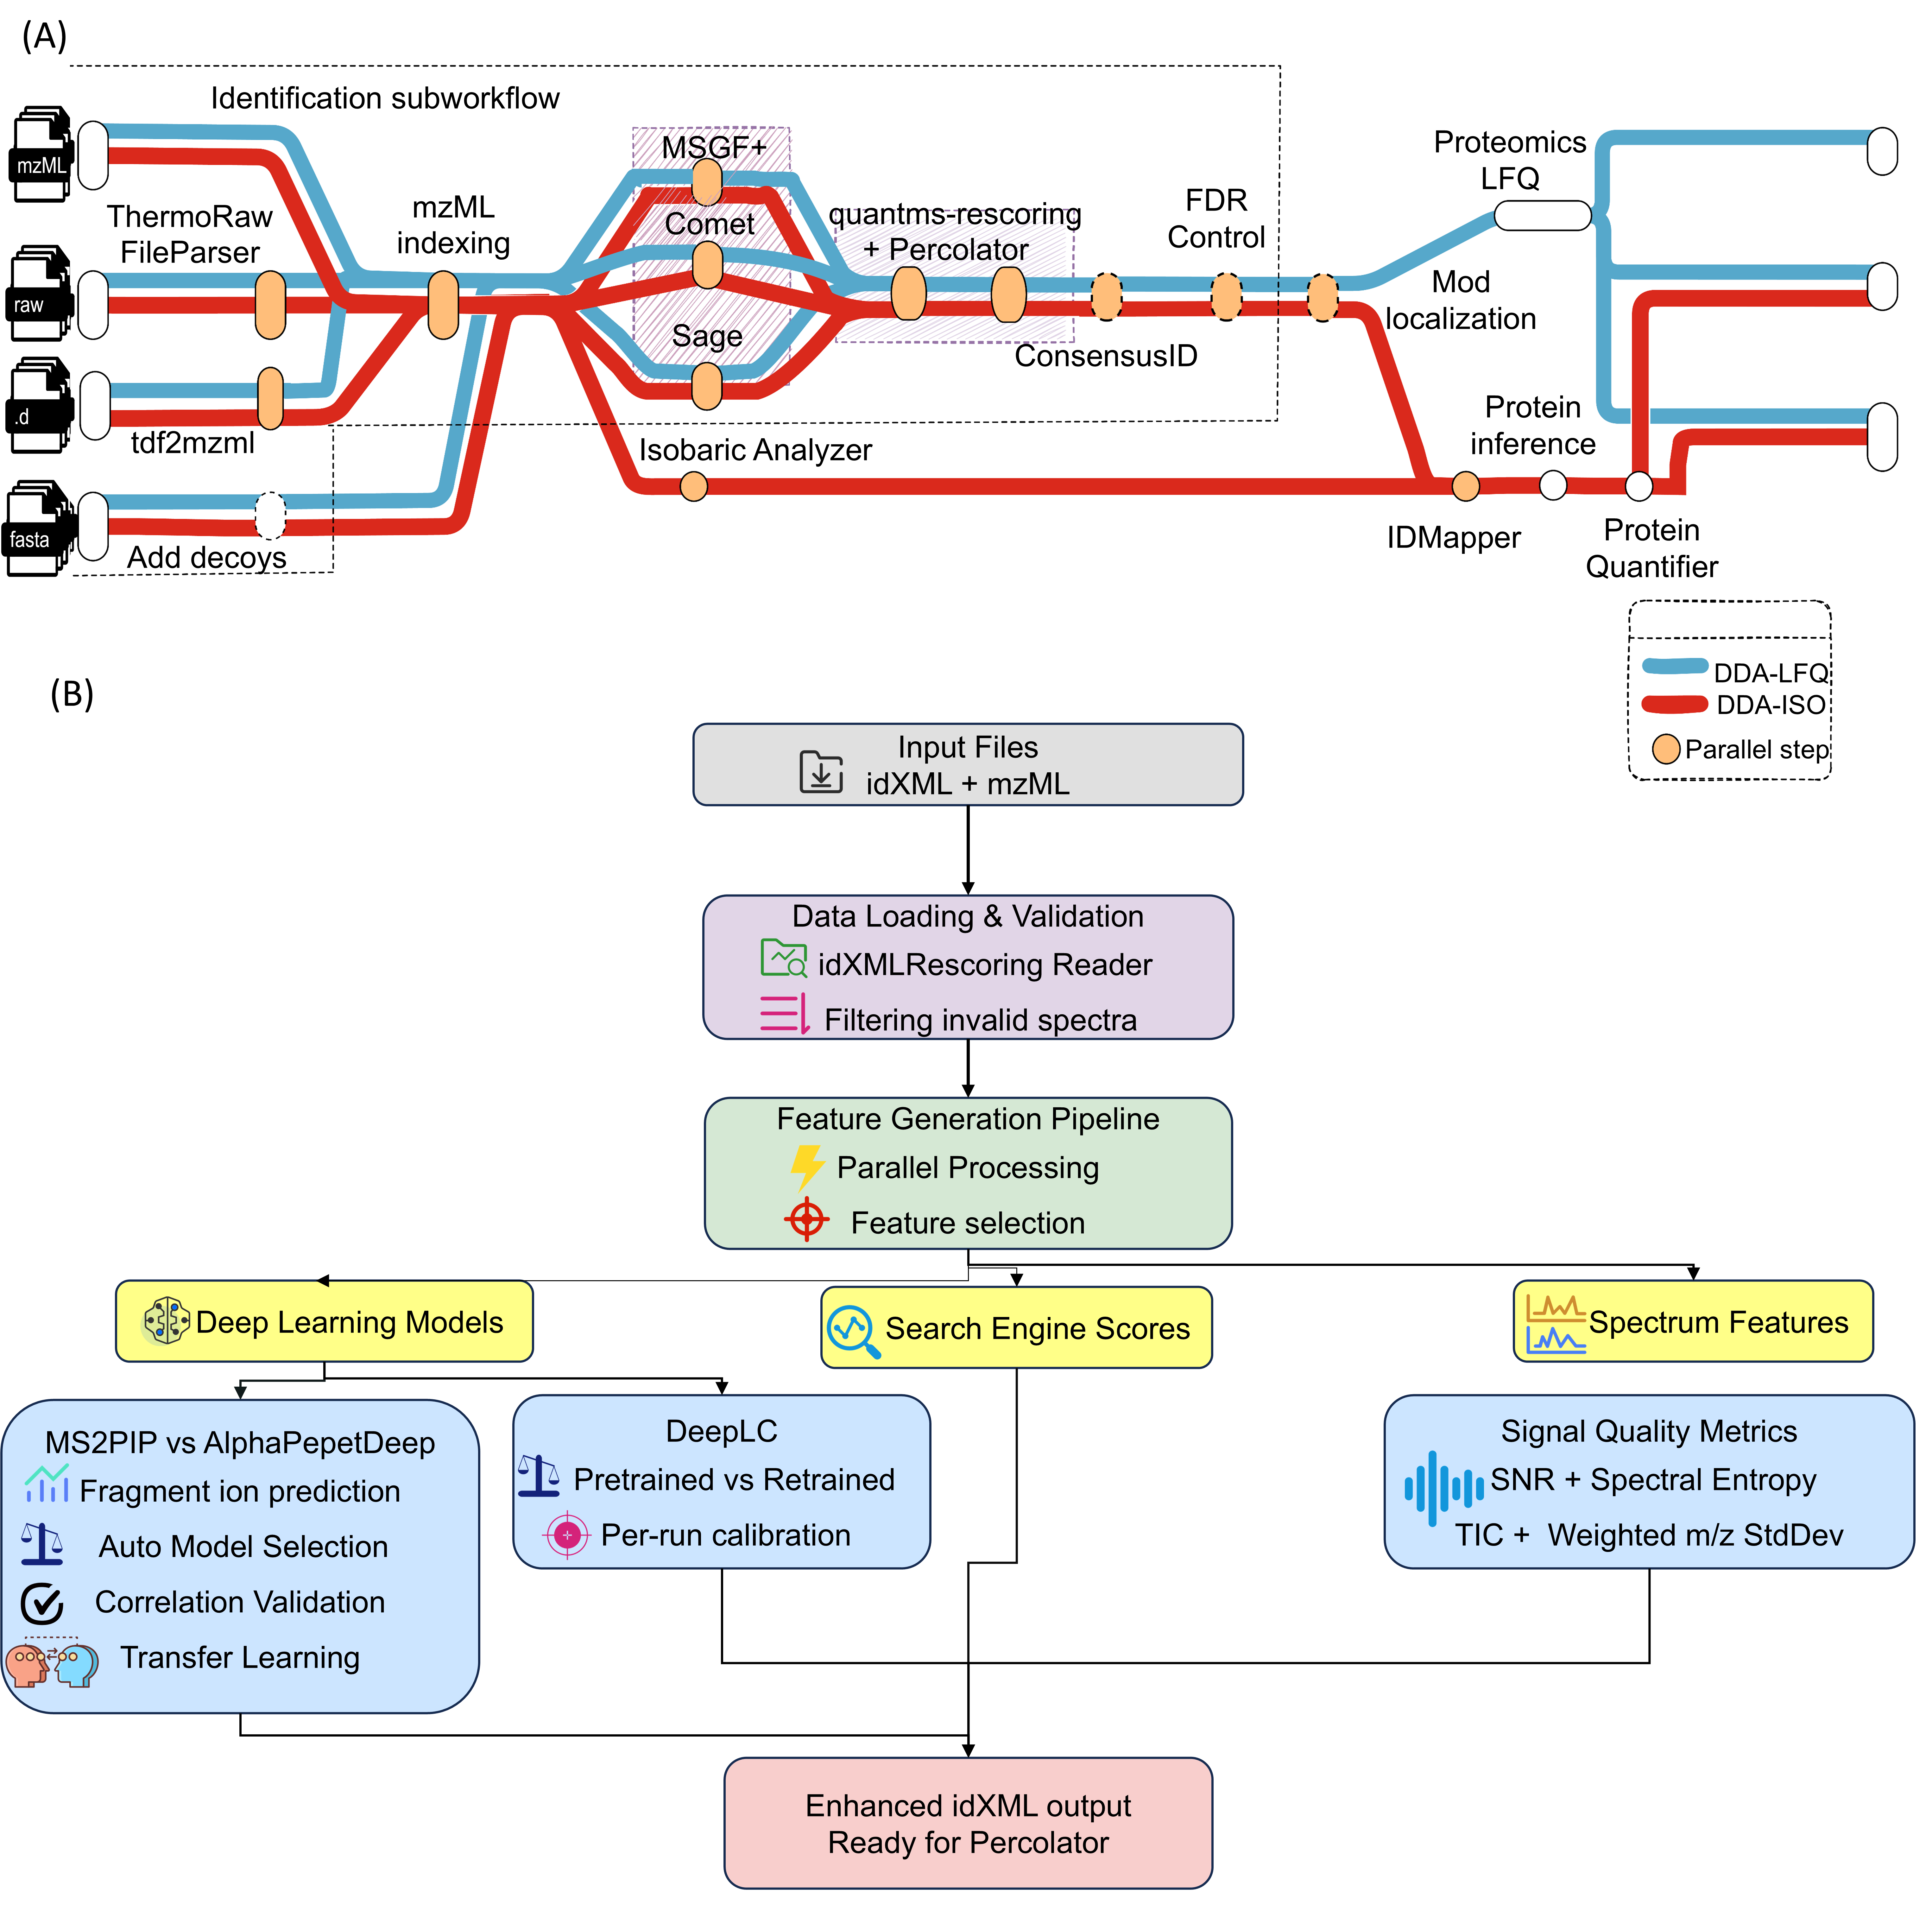
\includegraphics[width=1\textwidth]{figures//schema.png}
	\caption{The number of identified spectra as a function of differing FDR levels for different workflow settings. (A) Results for the PXD001819 dataset. (B) Results for the PXD001819 dataset showing protein quantification. Five different workflow settings are shown: the combination of Comet search engine with Percolator rescoring, the combination of Comet with MSGF+}
	\label{fig:schema}
\end{figure}

\section{Results}

\subsection{quantms with quantms-rescoring enhances LFQ identification and quantification}
To systematically evaluate the performance of the quantms-rescoring-enhanced workflow at both identification and quantification levels, we first analyzed the public UPS1 protein spike-in dataset PXD001819. For benchmarking the identifications, five different workflows configurations were designed and compared, including (1) Comet with Percolator, (2) two search engines with Percolator, (3) Comet with quantms-rescoring features and Percolator, (4) two search engines with quantms-rescoring features and Percolator, and (5) three search engines with quantms-rescoring features and Percolator to determine whether features from fragment intensity-based and retention time-based predictors improve sensitivity and specificity of identification and quantification.

To compare workflows, significant PSMs were filtered at varying FDR thresholds. As shown in Figure 1 ~\ref{fig:PXD001819_quantmsrescoring}, using consensus scores from two search engines significantly increased identification rates at a fixed FDR threshold. Specifically, combining Comet and MSGF+ improved identified spectra by 17\% over Comet alone, and incorporating MS²PIP and DeepLC features through quantms-rescoring led to an additional 16\% increase. quantms achieved a 28\% improvement in the number of PSM identifications compared to MaxQuant. At the quantification level, including quantms-rescoring–derived features allowed more low-abundance UPS1 proteins to be quantified (Figure 1B), highlighting the contributions of the integrated workflow. Although MaxQuant reported more UPS proteins in 250amol, 500amol and 2500amol, the proteins that were only quantified in MaxQuant were all quantified by match between runs (MBR) rather than from MS/MS. The main reason for this is that quantms used different MBR quality control. Therefore, we can observe that quantms achieved lower coefficients of variation (CV) than MaxQuant, considering only proteins that are quantified in at least 50\% of the replicates (Figure 1C-D). On the other hand, we also found that the variability of proteins quantified were not significantly reduced or increased after enabling quantms scoring. Together with the consistent rank–abundance patterns in Figure 2 and the lower replicate CVs (Figure 1C–D), these results support reliable quantification across UPS1 spike levels without requiring additional figures.

To better understand the contribution of individual features, we extracted the top 20 feature weights from Percolator (Figure S1). Over half of the top-weighted features were derived from quantms-rescoring. Notably, SpecPearsonNorm had a strong positive weight, indicating that a better correlation between predicted and observed intensities improves confidence. Conversely, RtDiffBest had a negative weight, suggesting that large deviations in retention time reduce match quality. Interestingly, peptide length also emerged as a significant positive feature after quantms-rescoring integration, likely because peptide length is an important feature as proxy to deterimine value of other specific features. For instance, for very short peptides, features like pearson correlation could be less valuable and should be ignored.

\begin{figure}[ht!]
	\centering
	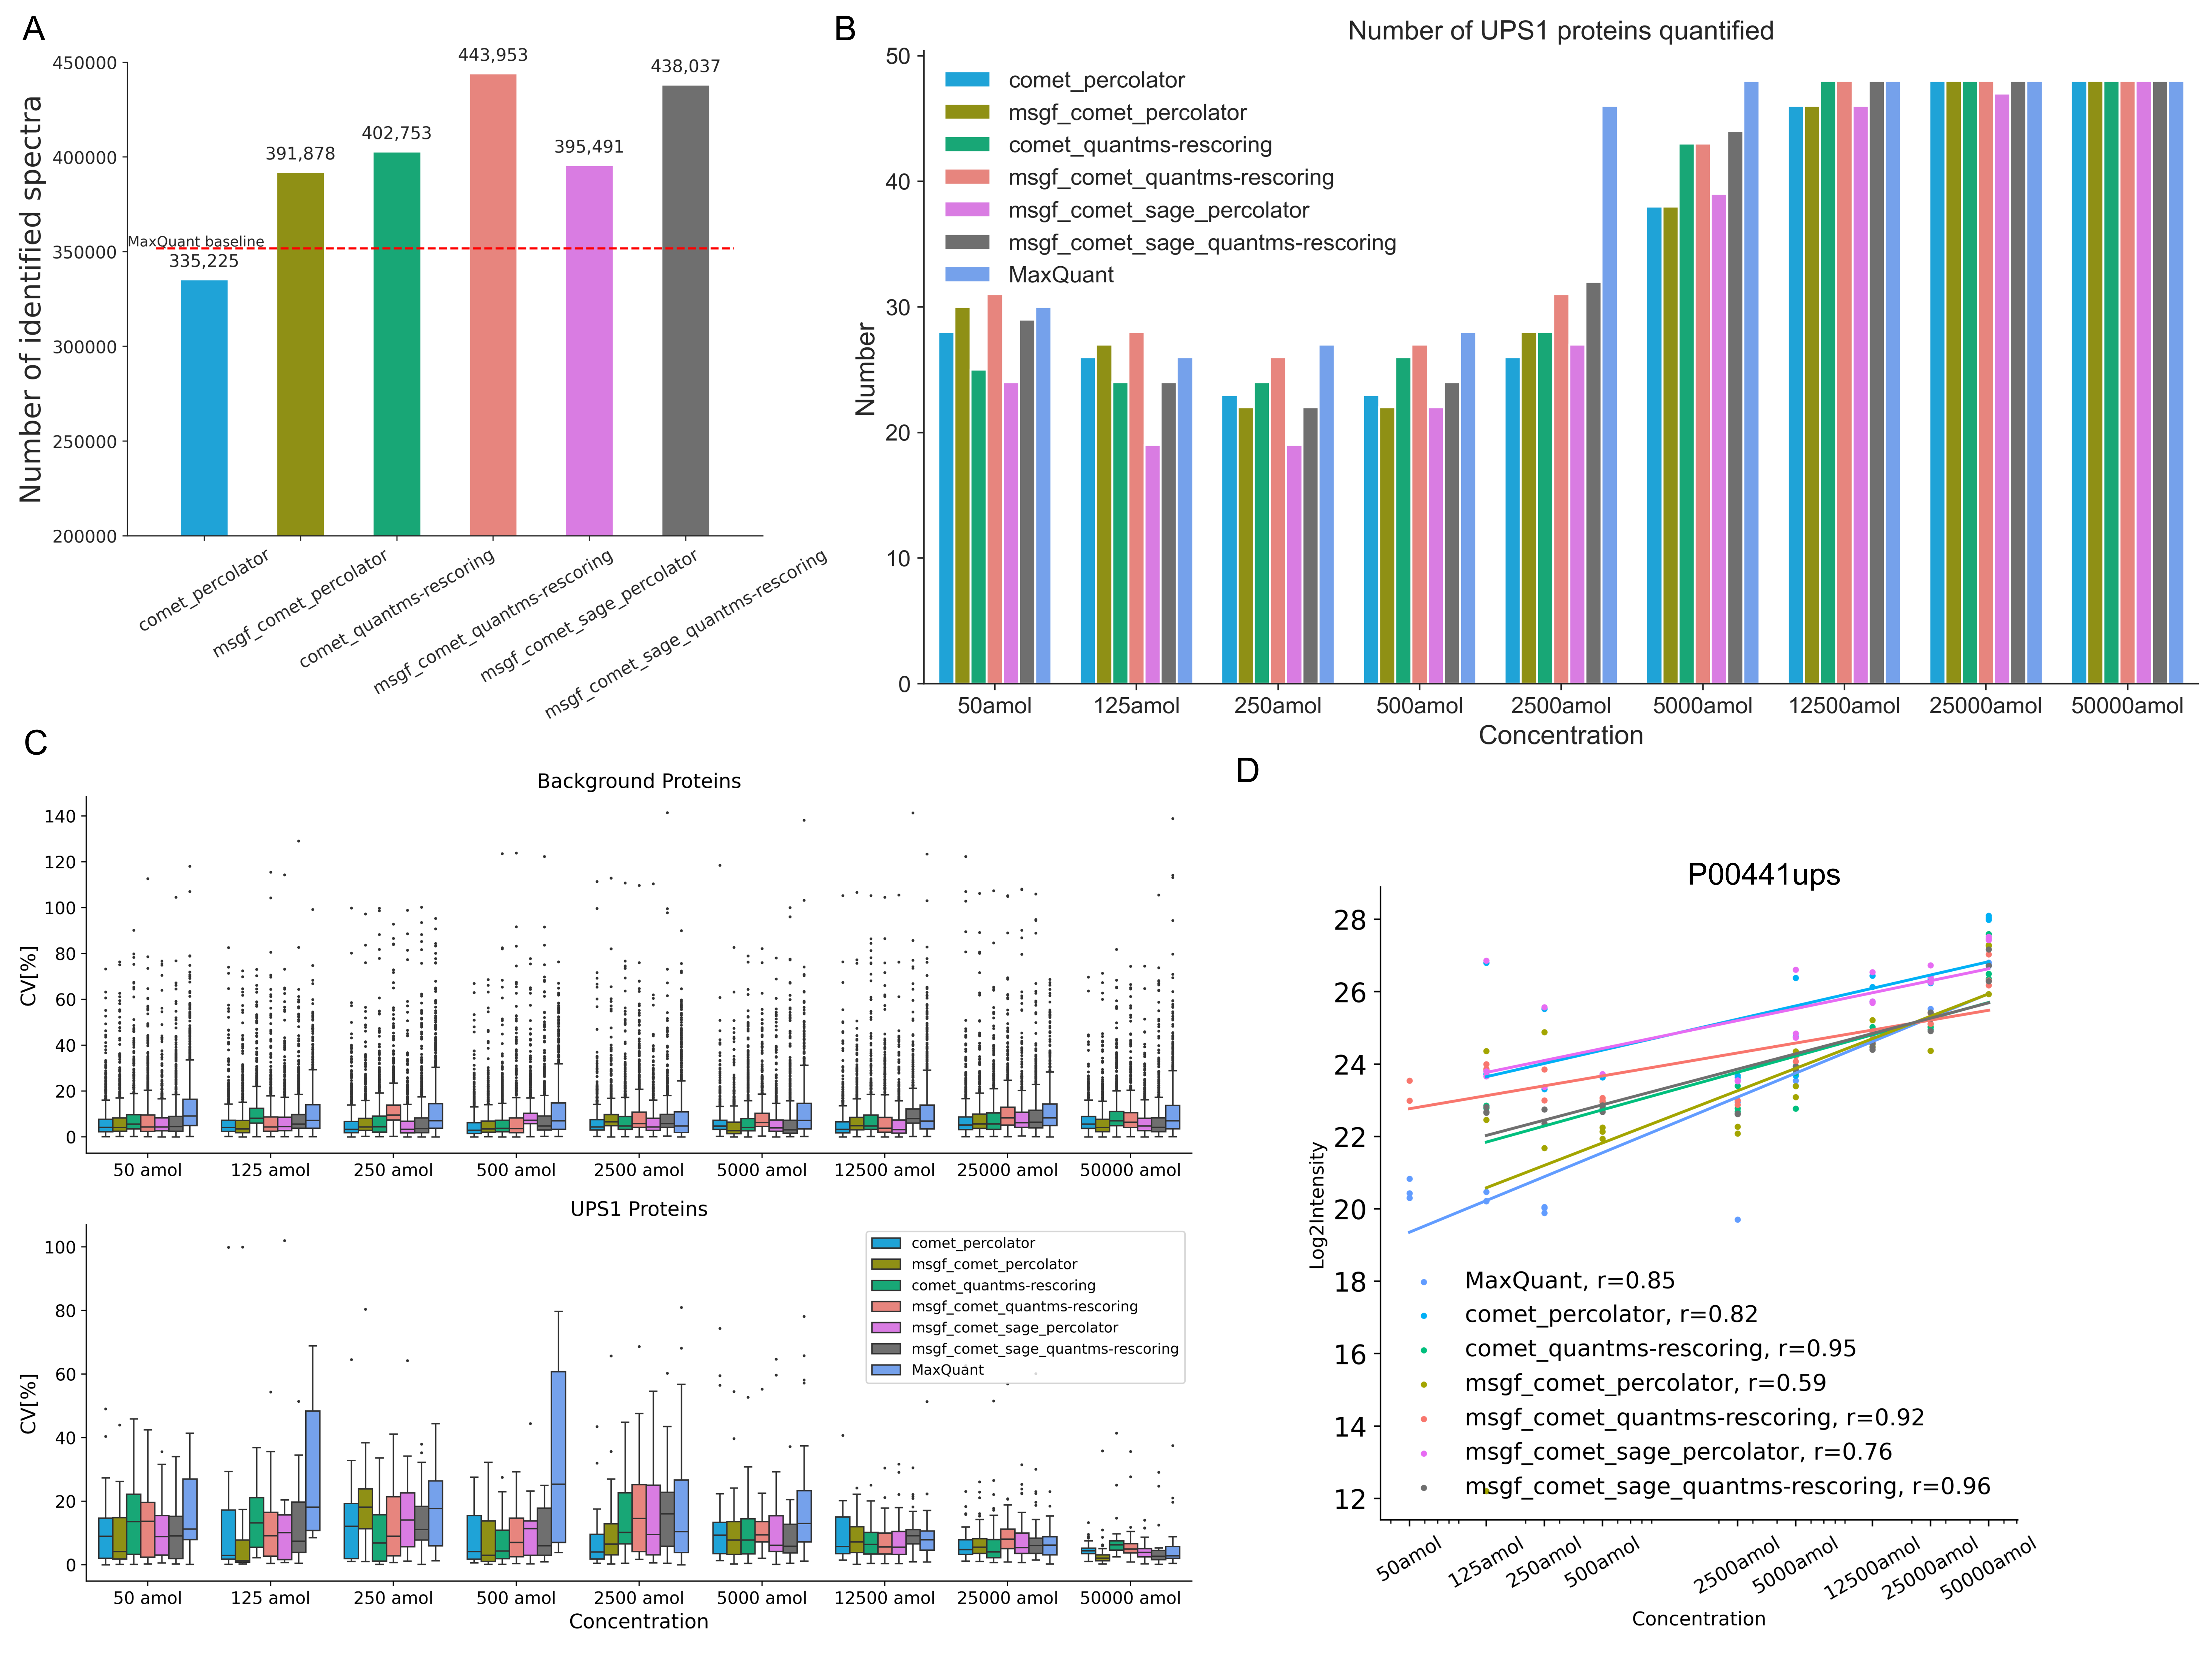
\includegraphics[width=1\textwidth]{figures//PXD001819_latest.png}
\caption{The number of identified spectra as a function of differing FDR levels for different workflow settings. (A) Results for the PXD001819 dataset. (B) Results for the PXD001819 dataset showing protein quantification. Five different workflow settings are shown: the combination of Comet search engine with Percolator rescoring, the combination of Comet with MSGF+, the combination of two search engines with quantms-rescoring features, the combination of two search engines with quantms-rescoring and SNR features, and the combination of three search engines with quantms-rescoring and SNR features. Multiple search engines consensus identification, additional intensity-based and retention time-based features, and SNR features lead to both higher identification rates and high-quality identification. Coefficient of variation of Yeast (C) and UPS1 proteins (D) for the reanalysis of PXD001819 using MaxQuant and quantms with different configurations.}
\label{fig:PXD001819_quantmsrescoring}
\end{figure}

\subsection{Improved identification and quantification in tandem mass tag (TMT) experiments via quantms-rescoring}
We next applied the workflow to a large-scale TMT-labeled dataset from the Clinical Proteomic Tumor Analysis Consortium (CPTAC; PDC000127). The integration of multiple search engines and quantms-rescoring led to substantial improvements in both identification and quantification (Figure~\ref{fig:PDC_quantmsrescoring}). In Figure 2A–B, we compare Comet+MSGF+ with Percolator versus the same workflow with quantms-rescoring; the PSM identification rate increased by 3.6\% and 921 proteins were newly quantified relative to the workflow without quantms-rescoring.

Among these, 59 proteins had abundance levels within the top 10\% (Figure 2C). To assess the biological impact of rescoring, we conducted differential expression analysis using the quantms-rescoring–enhanced workflow. As shown in Figure 2D, 27 newly quantified proteins were significantly differentially expressed. Notably, FOXG1—one of these proteins—has been associated with prognosis in Clear Cell Renal Cell Carcinoma, as reported by Yang et al. \cite{yang_comprehensive_2022}. These findings illustrate that quantms incorporating MS²PIP and DeepLC-derived features enhances not only identification sensitivity but also enables deeper biological insights.

We further examined the rescoring contribution of individual features by analyzing the top 20 support vector machine (SVM) weights from Percolator (Figure S2). For Comet-based results, SpecPearsonNorm, DotProdIonYNorm, and RtDiffBest were highly weighted. The interpretations of these weights were consistent with those from the label-free dataset. Importantly, peptide length again emerged as a key feature. Similar weight distributions were observed for MSGF+ and SAGE results, confirming the generalizability of these feature effects across different search engines. (Supplemental Figure~\ref{fig:PDC_Go_EA})

\begin{figure}[ht!]
	\centering
	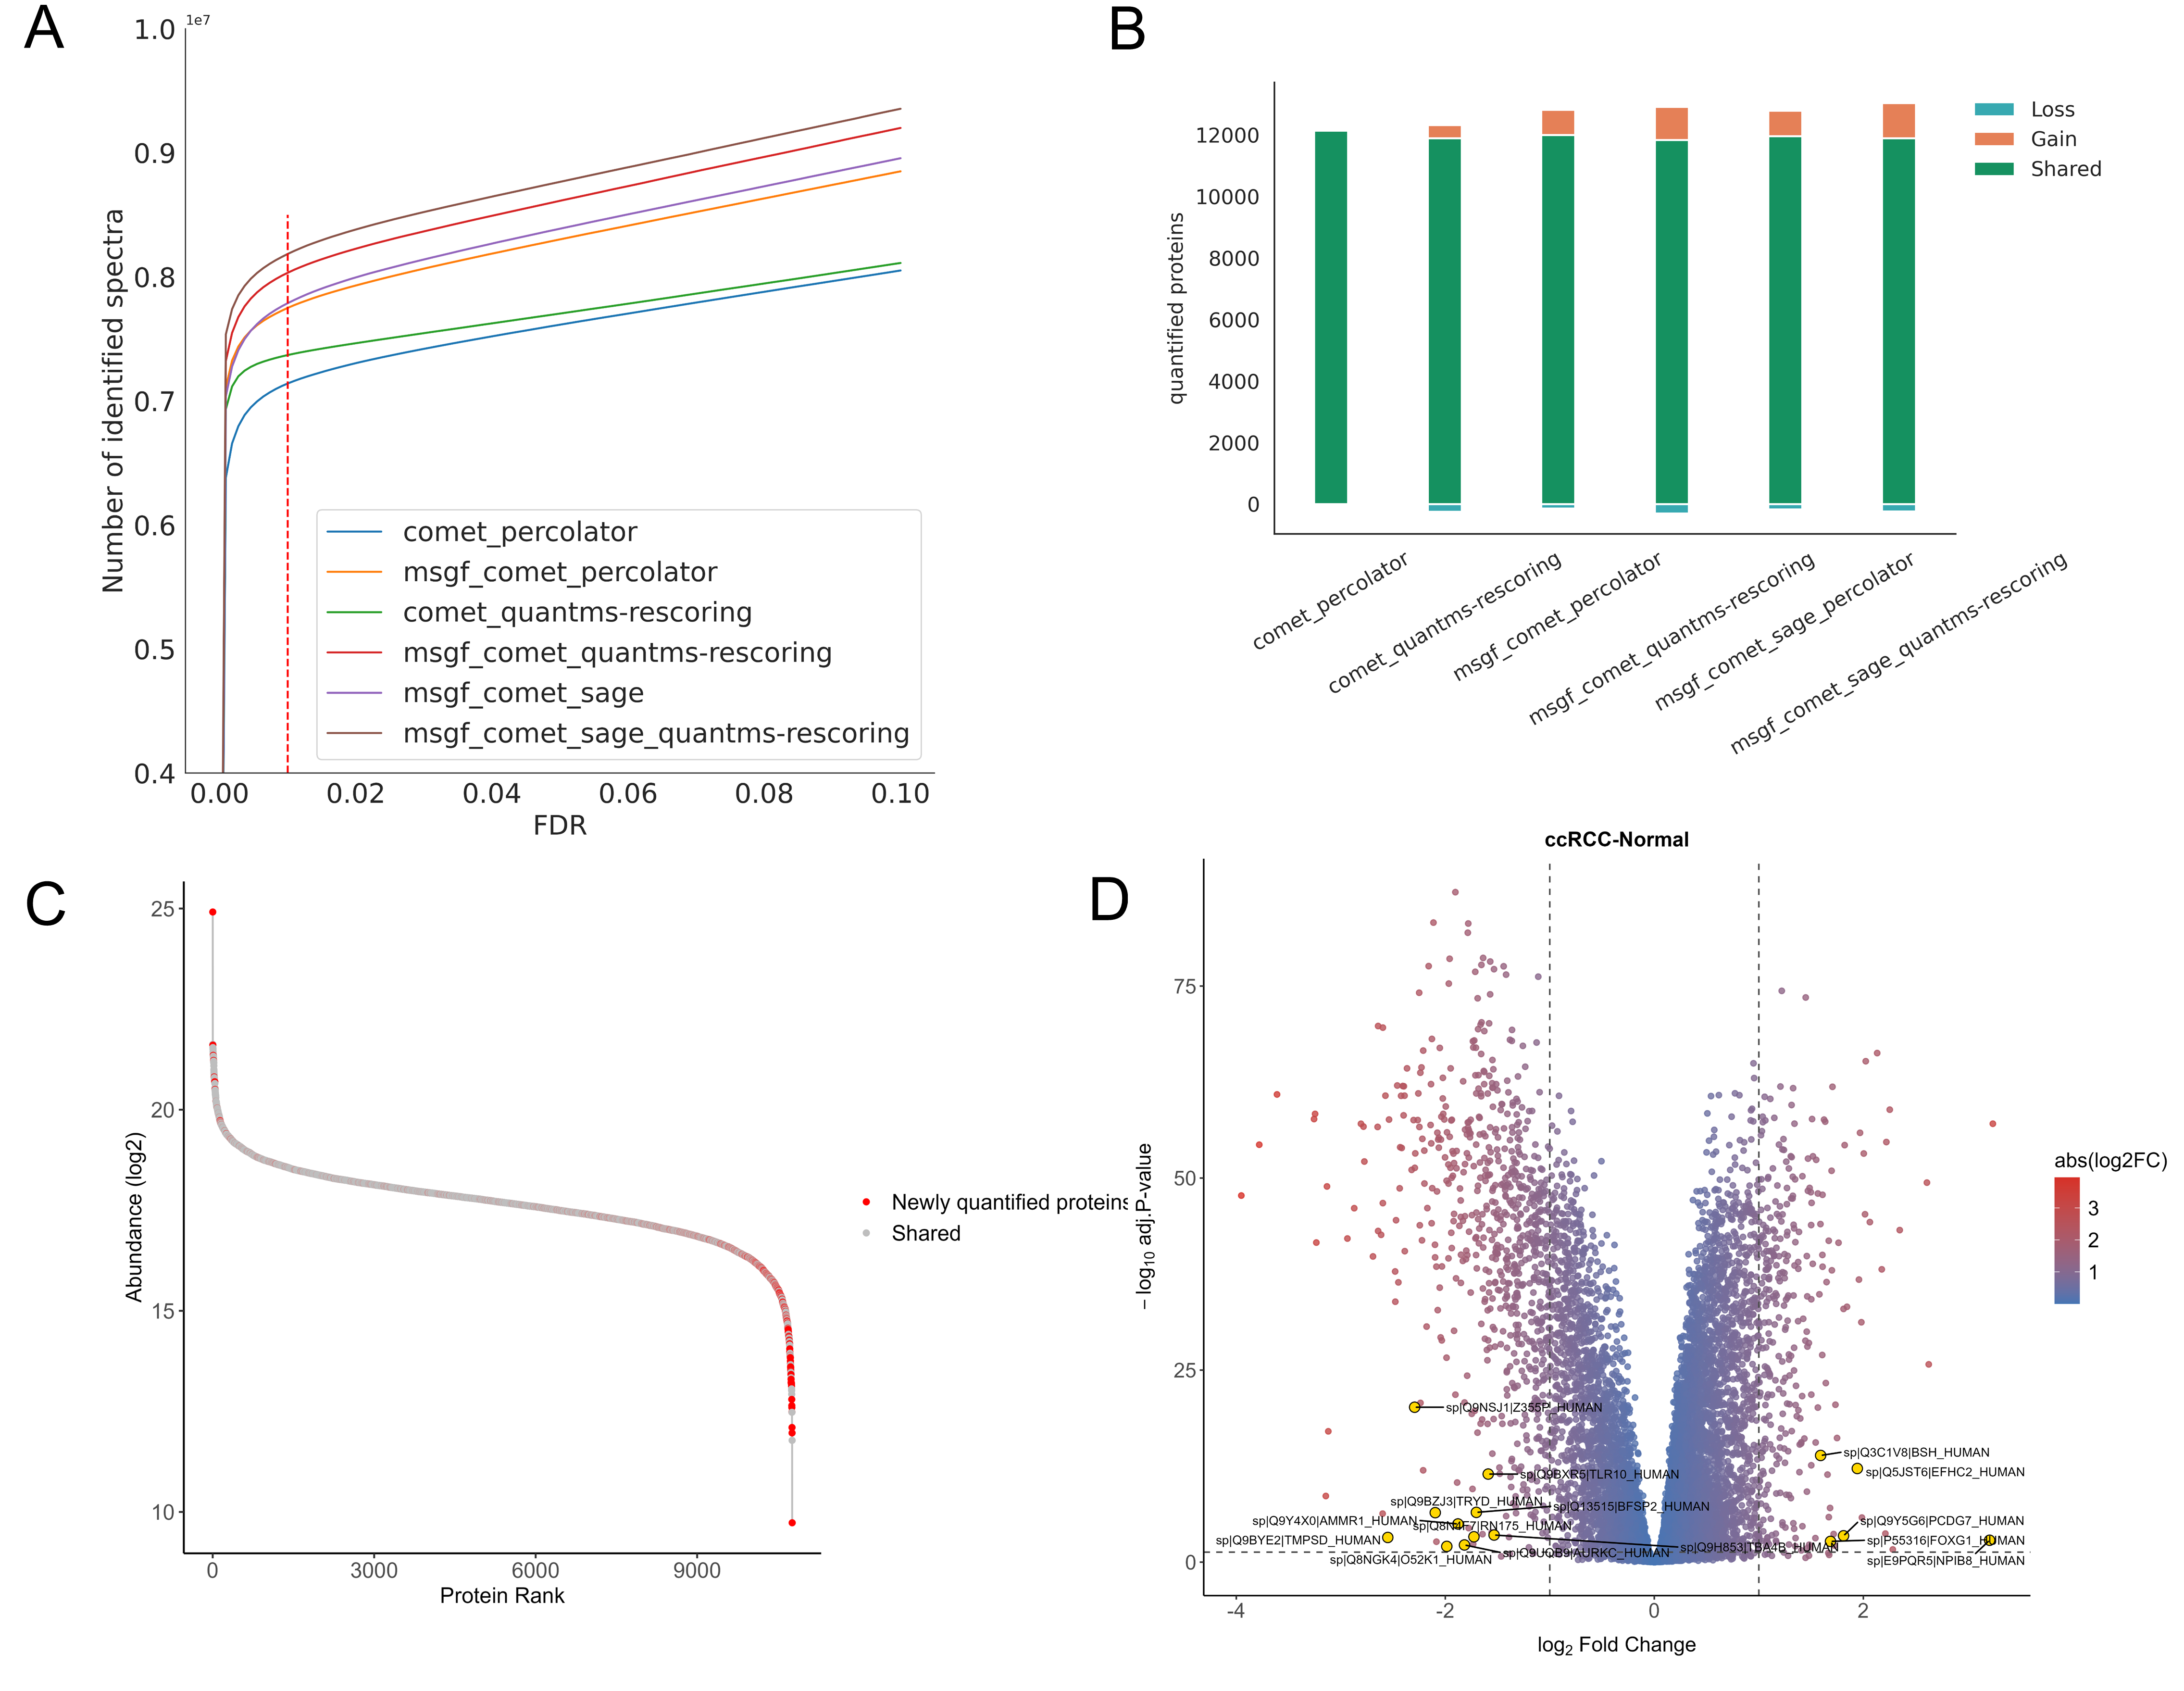
\includegraphics[width=1\textwidth]{figures//CPTAC_latest.png}
\caption{Comparison on PDC000127. Panels A–B compare Comet+MSGF+ (Percolator) versus Comet+MSGF+ with quantms-rescoring: (A) identified spectra across FDR levels; (B) number of quantified proteins. (C) Rank of protein abundance for Comet+MSGF+ with quantms-rescoring; red dots indicate proteins unique to the rescoring workflow vs without. (D) Volcano plot from MSstatsTMT; yellow dots indicate proteins quantified only in the rescoring workflow vs without.}
\label{fig:PDC_quantmsrescoring}
\end{figure}


\subsection{quantms with quantms-rescoring improves immunopeptidome identification}
The HLA Ligand Atlas \cite{marcu_hla_2021} (PXD019643) is a comprehensive map of HLA-I and HLA-II-presented peptides from 30 benign tissues, 51 HLA-I alleles, and 86 HLA-II alleles. To further assess the performance of the quantms workflow using quantms-rescoring, we analyzed the HLA Class II data of the HLA Ligand Atlas. Five workflow configurations were evaluated: (1) Comet with Percolator, (2) Comet with quantms-rescoring, (3) Comet and MSGF+ with Percolator, (4) Comet and MSGF combined with quantms-rescoring features, and (5) Comet and MSGF+ combined quantms-rescoring/SNR features, displayed in Figure4 ~\ref{fig:PXD019643_figure4}. 
 
With local peptide-level FDR threshold of 1\% among the technical replicates per sample, integrating MSGF+ with Comet increased the number of identified peptide by 1.6\% compared to using Comet alone. Adding quantms-rescoring features on top of Comet workflow yielded a further 14\% improvement compared to MSGF+ with Comet workflow. Enabling the quantms-rescoring combined with MSGF+ and Comet, the peptide identification improved by an additional 5\% compared to workflows using only Comet and quantms-rescoring. When considering spectra features such as SNR in Supplementary Table S1, the peptide identification improved by an additional 0.6\% compared to workflows using MSGF+, Comet and quantms-rescoring.
To demonstrate the application potential of the quantms pipeline for antigen discovery, we show the number of HLA class II peptides predicted as binder (Figure 4B,C and D). Added quantms-rescoring features to the Comet workflow, enabling the identification of 8,867 additional binding. When quantms-rescoring was enabled in combination with MSGF+ and Comet, an additional 2,821 binding were identified. And the length distributions of HLA class II peptide binders predicted are consistent by different workflows configurations. It displays a local maximum occurring at approximately 15-mers (Figure 4E). In addition, using local PSM-level FDR threshold of 1\%, integrating MSGF+ with Comet increased the number of identified spectra by 11.7\% compared to using Comet alone. Adding quantms-rescoring features on top of the multi-engine workflow yielded a further 22.8\% improvement (Figure S3).

To better understand the impact of quantms-rescoring-derived features on rescoring, we visualized the distributions of decoy PSMs, rejected target PSMs, and accepted target PSMs using the Pearson correlation coefficient (PCC) and retention time error (Figure S3C,D). The accepted target PSMs were clearly separated from both decoy and rejected targets based solely on PCC values, and exhibited consistently low retention time deviations. The top 20 feature weights from Percolator are displayed in Figure S4. The features of the MSGF+ search engine carry significant weight, such as SpecEValue, which indicates that when only MSGF+ is used, the gain of quantms-rescoring is limited. However, features from quantms-rescoring occupy a larger weight for Comet search engine, including 9 MS²PIP and 2 DeepLC features. This further illustrates that using consensus identifications by multiple search engines helps to coordinate the differences between different search engines. 
Overall, these results demonstrate the robustness of the quantms workflow in immunopeptidomics, highlighting its ability to leverage machine/deep learning learning-derived features to maximize identification accuracy through multi-engine consensus rescoring.

\begin{figure}[ht!]
	\centering
	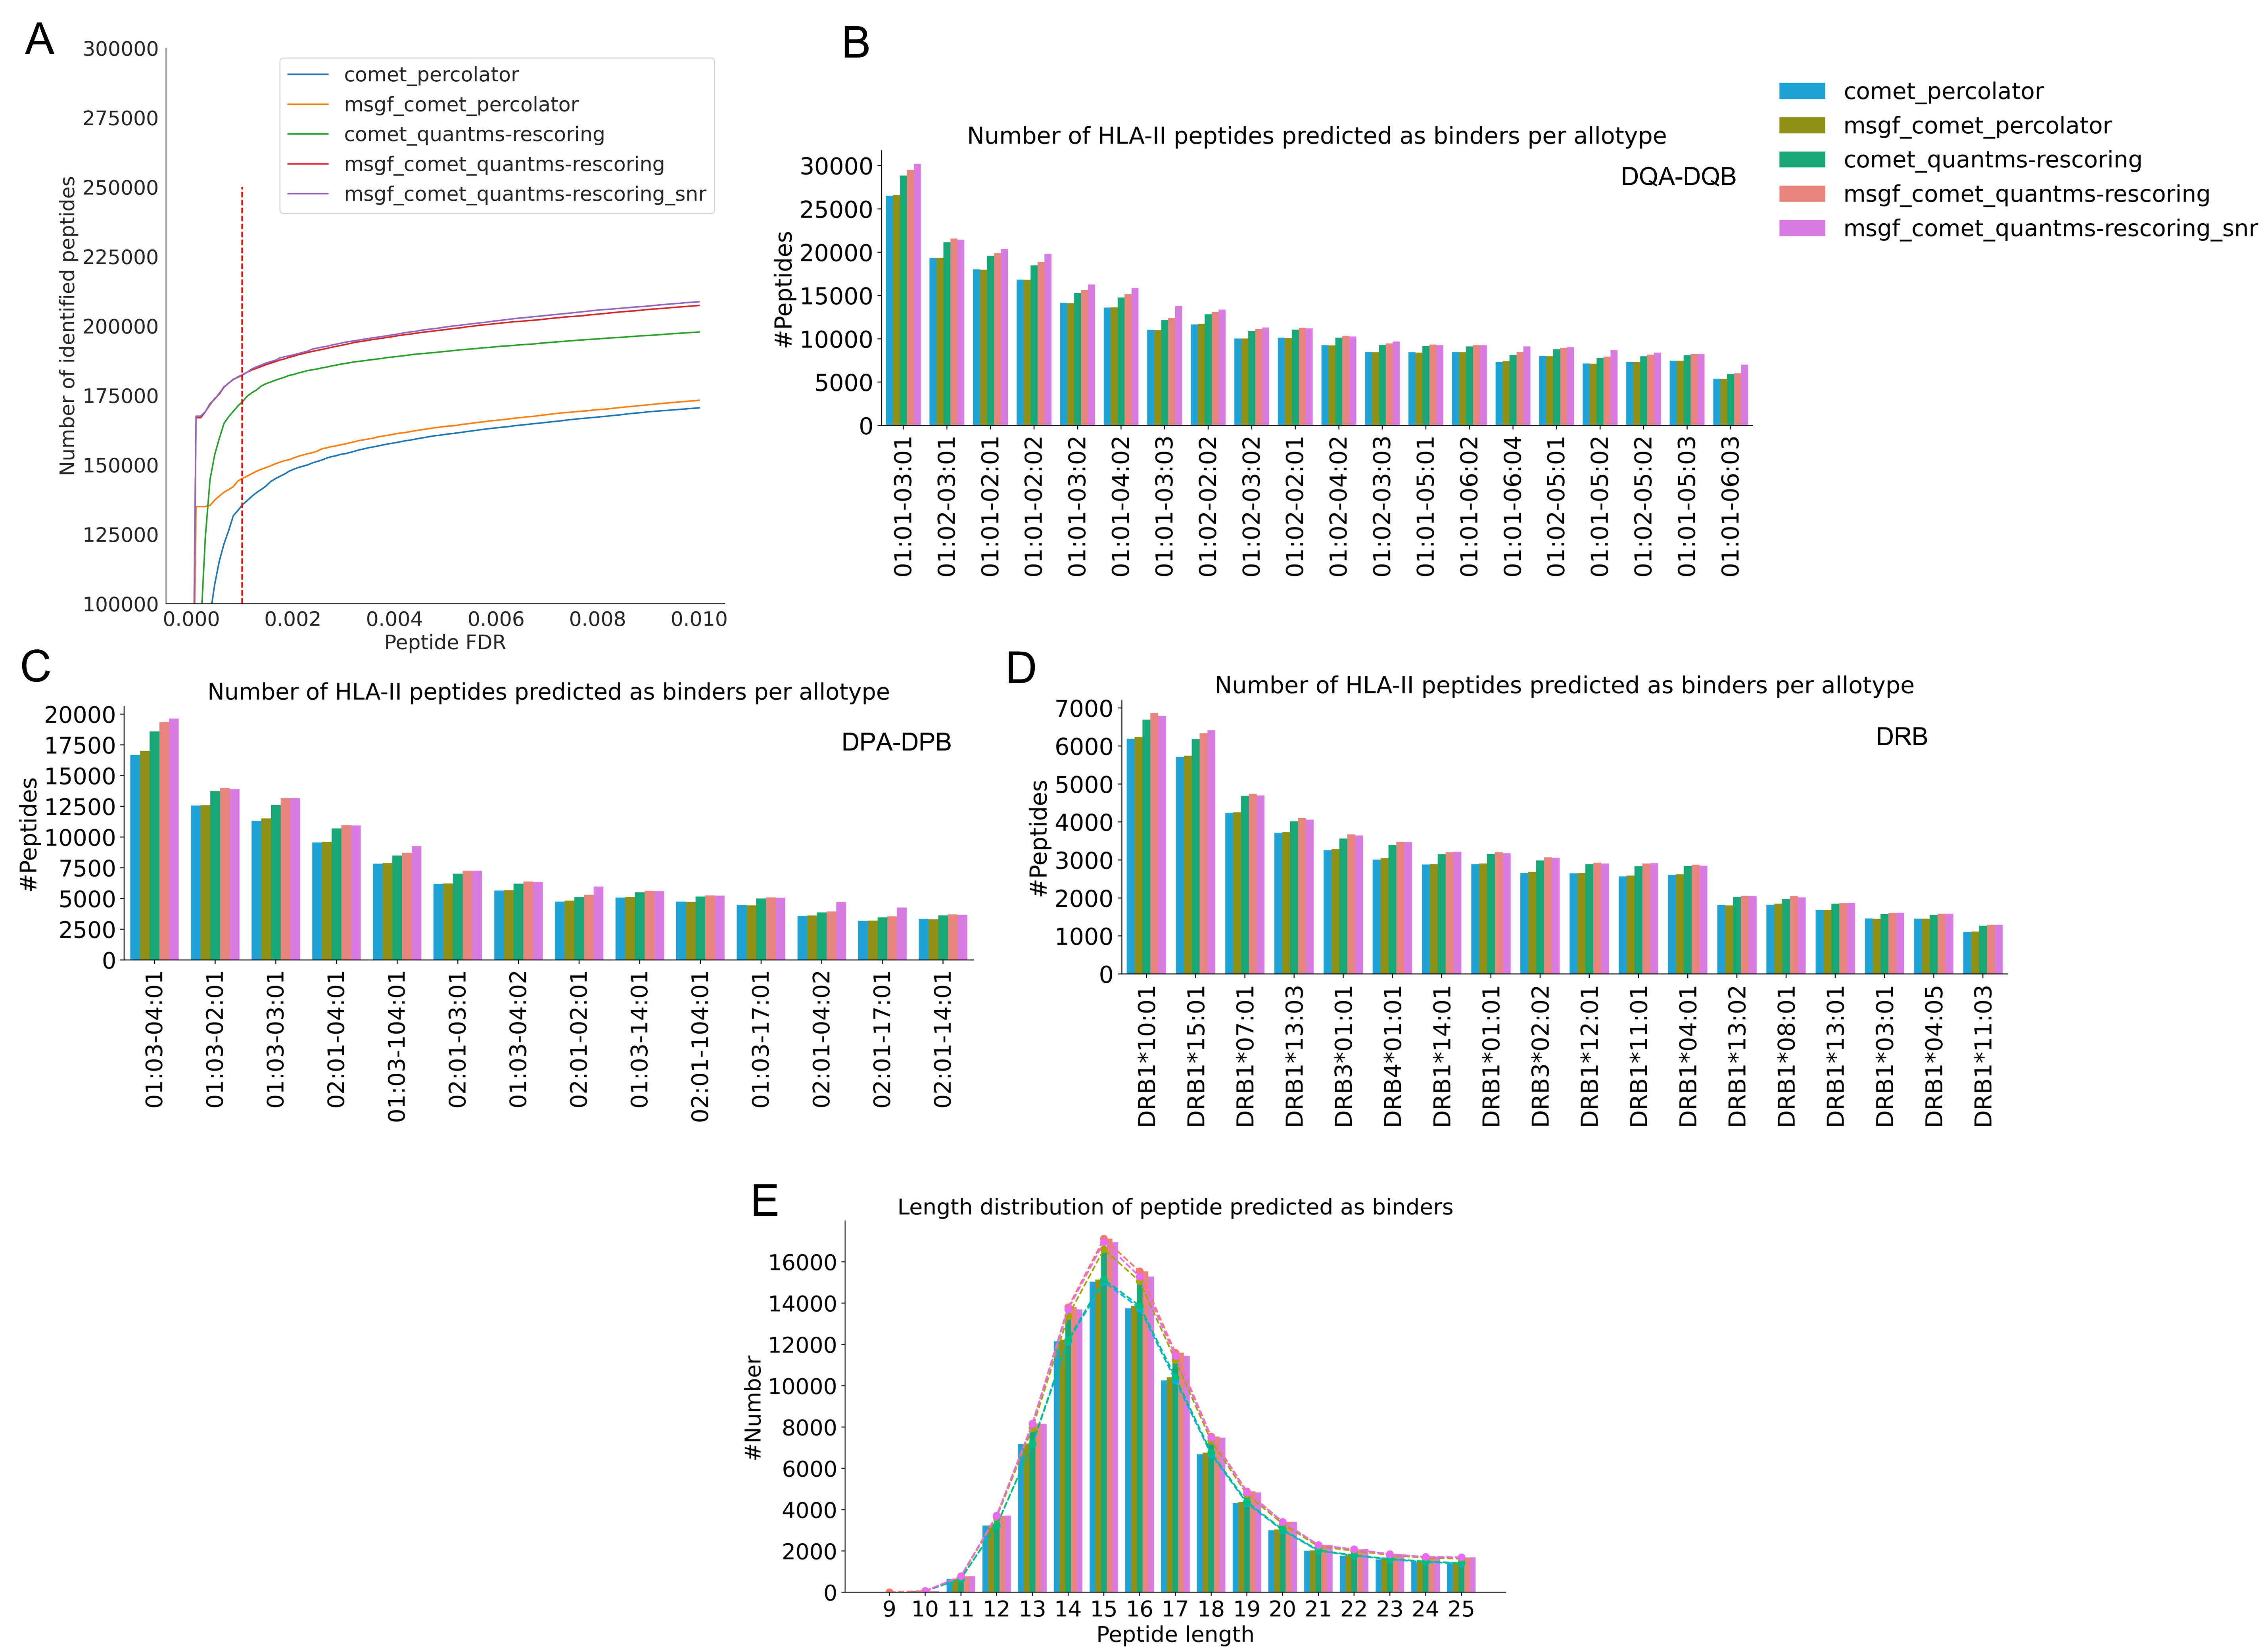
\includegraphics[width=1\textwidth]{figures//PXD019463_figure4.png}
	\caption{Comparison of immunopeptides identification results for different workflow settings on PXD019643. (A) Line plot showing the number of peptide identified for four workflow settings at different peptide FDR levels. (B, C, D) Global overview of HLA-II predicted binders distributed across HLA molecules. HLA binding prediction was performed with NetMHCIIpan-4.3(\% binding rank $\leq$ 5). (E) Length distribution of identified HLA-II peptides predicted as binders from all samples was analyzed.}
	\label{fig:PXD019643_figure4}
\end{figure}

\subsection{Enhanced Phosphopeptide Identification and Localization Using quantms-rescoring}
In addition, we investigated the performance of our quantms workflow with quantms-rescoring on post-translational modification experiments (PXD026824). For phosphoproteomics analyses, different workflow settings were evaluated: (1) Comet + Percolator, (2) Comet + quantms-rescoring, (3) Comet + MSGF+ + Percolator, and (4) Comet + MSGF+ + quantms-rescoring features. As shown in Figure~\ref{fig:PXD026824_quantmsrescoring}, combining search engine consensus results with quantms-rescoring features substantially improves Percolator's ability to discriminate between true and false PSMs. This is evident from the leftward shift in score distributions compared to the Comet-only workflow, indicating improved stringency (Figure 4A). Specifically, incorporating quantms-rescoring features into the two-search-engine consensus increased the number of identified spectra by 24\% compared to consensus identification alone. Previous research suggest that phosphorylated peptides may produce -98 Da phosphoric acid neutral losses. Therefore, we further evaluate the impact of considering neutral loss on re-scoring performance when calculating features. quantms-rescoring with modloss ions increased the number of identified spectra by 3\% compared to without modloss ions. The top 20 feature weights from Percolator, displayed in Supplementary Figure~\ref{fig:phospho_features}, highlight the consistent importance of features such as IonYNorm and DotProdIonYNorm, similar to previous datasets.

Given the importance of false localization rate (FLR) control in phosphoproteomics, we also assessed the impact of different workflows on phosphopeptide identification at varying false localization rate (FLR) thresholds (Figure 4B, C). After filtering with PSM FDR 0.01 and local FLR 0.01, the consensus workflow with quantms-rescoring features identified 20\% and 23\% more phosphorylated peptides than its counterpart without quantms-rescoring and single search engine. Notably, after filtering with PSM FDR 0.01, FLR 0.01 and protein FDR 0.01, 1,809 phosphorylated peptides were uniquely quantified by the quantms-rescoring enabled workflow compared to without quantms-rescoring. When considering -98 Da neutral losses, 2,191 phosphorylated peptides were uniquely quantified compared to without quantms-rescoring. At the phosphosite level, workflow with quantms-rescoring also uncovered 842 novel protein phosphorylation sites not reported in the other workflow configuration without quantms-rescoring (Figure 4D), and an additional 495 novel protein phosphorylation sites are reported when considering -98 Da neutral losses. Collectively, these results underscore the value of quantms-rescoring in enhancing both identification sensitivity and site-level localization in phosphoproteomics, establishing quantms as a robust solution for large-scale PTM data analysis.

\begin{figure}[ht!]
	\centering
	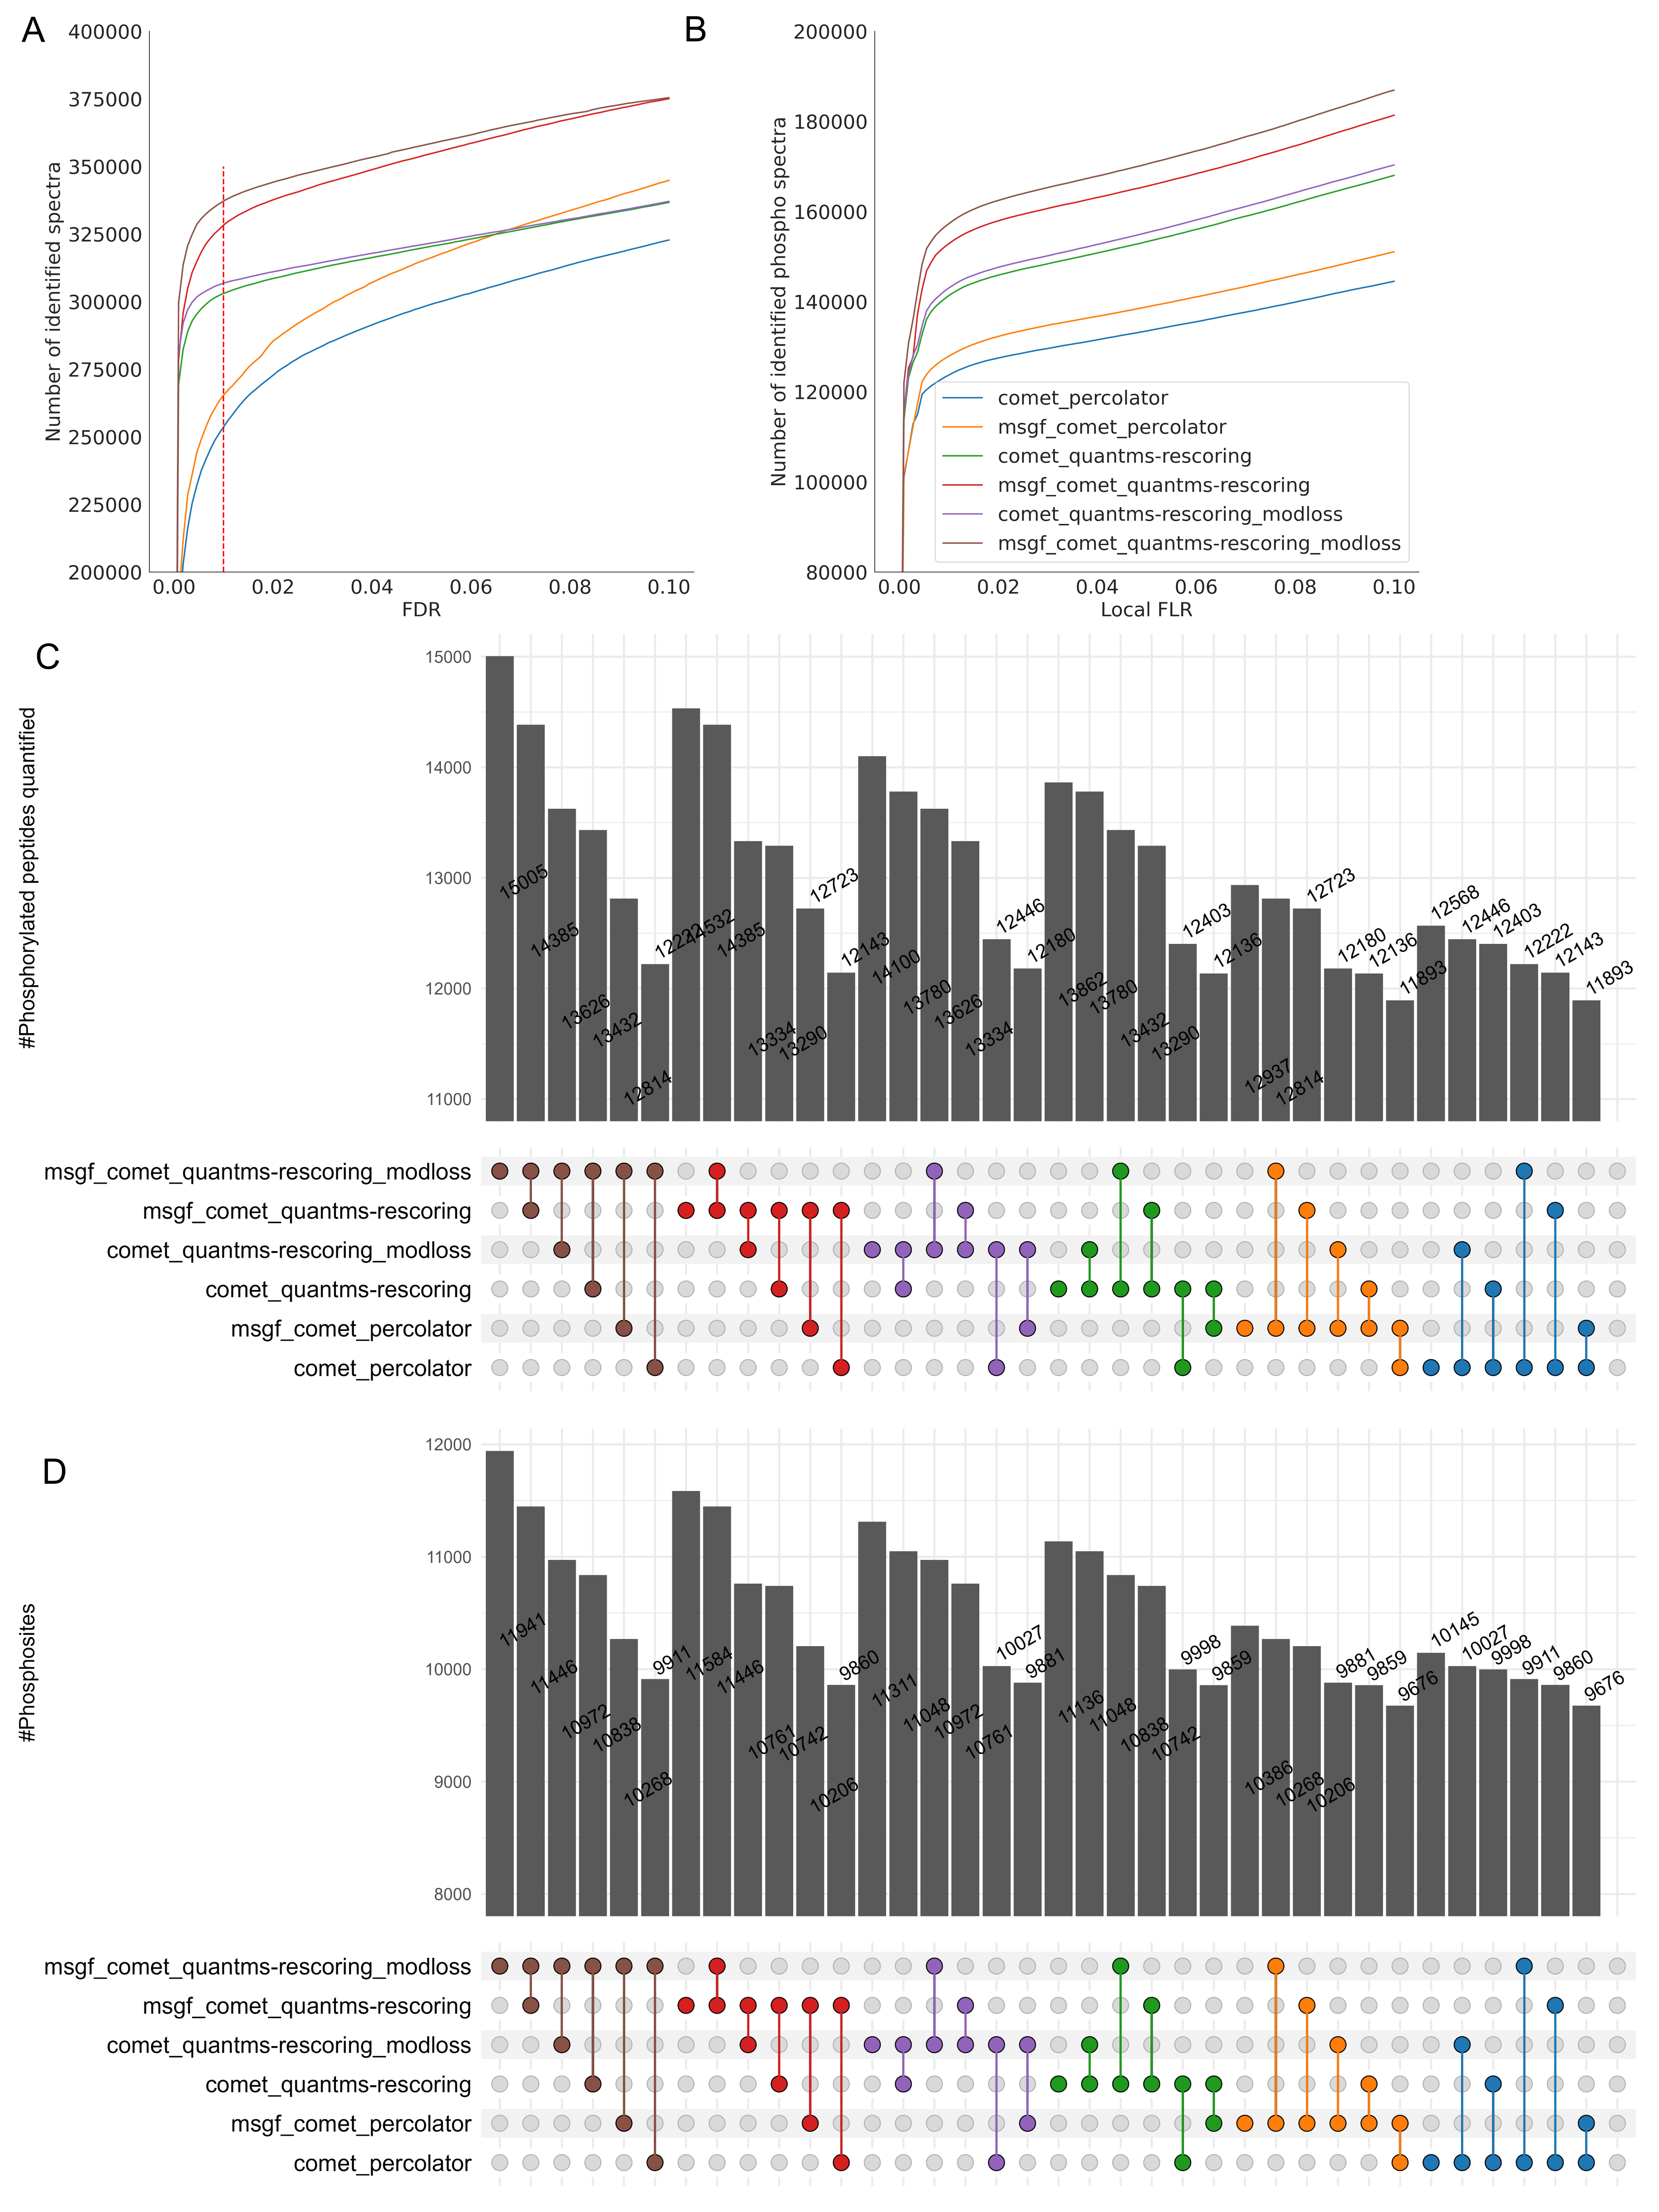
\includegraphics[width=1\textwidth]{figures//phospho4.png}
	\caption{Comparison of phosphorylated peptide identification results for different workflow settings on PXD026824. (A) Line plot showing the number of spectra identified for four workflow settings at different PSM FDR levels. (B) Line plot showing the number of phosphorylated spectra identified for four workflow settings at different local false localization rate levels after an FDR of less than 0.01 at the PSM level. (C) Venn diagram of peptides quantified for four settings. (D) Venn diagram of protein phosphosites at protein FDR 0.01 and FLR 0.01 for four settings.}
	\label{fig:PXD026824_quantmsrescoring}
\end{figure}


\section{Discussion}
Advancements in deep learning-based tools have significantly improved the sensitivity of peptide-spectrum match (PSM) rescoring, yet their integration into streamlined, reproducible, and quantitative, scalable proteomics workflows has remained limited, especially for large-scale public data analysis. In this study, we demonstrate the systematic incorporation of quantms-rescoring into the open-source quantms pipeline and evaluate its impact across various experimental settings, including label-free quantification (LFQ), tandem mass tag (TMT)-based quantification, immunopeptidomics, and phosphoproteomics. Our results show that enhanced feature sets derived from MS²PIP and DeepLC not only increase the identification rates but also improve the quantification depth. 

Importantly, we provide evidence that the improved identification process via rescoring propagates downstream into quantification, leading to increased numbers of proteins with reliable abundance estimates, as well as enhanced detection of differentially expressed proteins, and enhanced localization of PTMs. These findings are in line with prior work on MHCquant2 \cite{scheid2025mhcquant2}, which showed that adding MS²Rescore to Comet improves sensitivity in immunopeptidomics and that moving from a single‑engine setup to a multi‑engine consensus further increases PSM counts; our multi‑engine results corroborate this trend.

To demonstrate the applicability and advantages of quantms integrated with quantms-rescoring in quantitative proteomics, we performed a series of reanalyses using publicly available large-scale datasets with well-established benchmarks. In label-free experiments, quantms-rescoring–enhanced workflows achieved significant increases in PSM and peptide identification rates while maintaining or improving quantification reproducibility across replicates. For TMT experiments, the integration of quantms-rescoring into quantms increased the number of quantifiable proteins. In more challenging applications, such as immunopeptidomics and phosphoproteomics, the deep learning-based rescoring pipeline consistently yielded higher identification rates and improved sensitivity.
These improvements will contribute to meaningful biological insights, such as phosphosite discovery and the identification of differentially expressed proteins with potential clinical relevance. In addition, we counted the run times with different configurations and the added sensitivity from rescoring does add 15\%-50\% of run time, as shown as Supplementary Table ~\ref{tab:resources_stats}. This overhead can be mitigated in practice by increasing Nextflow executor parallelism for quantms-rescoring and leveraging large cloud-based or high-performance computing (HPC) architectures, which we used to maintain throughput on large datasets.

Overall, the results highlight the synergistic benefits of integrating machine learning-based features within end-to-end, cloud-based proteomics workflows. By embedding quantms-rescoring into the quantms pipeline, we provide a practical and accessible solution for the community to leverage cutting-edge spectral prediction and retention time modeling without the need for complex manual configuration. This integrated approach enables reproducible reanalysis of large public datasets, increases identification confidence, and strengthens quantitative conclusions across diverse experimental designs.

\section*{Data availability}
All datasets analyzed in this study are publicly available. Raw data and metadata can be obtained from the PRIDE Archive under the accessions PXD001819 (LFQ benchmark), PXD019643 (immunopeptidomics), and PXD026824 (phosphoproteomics), and from the CPTAC data portal under PDC000127 (TMT). Sample and Data Relationship Files (SDRFs) used in this work are available in the project repository at \url{https://github.com/bigbio/quantms-rescoring-paper}. Where applicable, additional configuration files and parameters are included alongside the SDRFs to facilitate reuse. quantms-rescoring is open source and available at \url{https://github.com/bigbio/quantms-rescoring}.

\section*{Acknowledgments}
We thank all those who supported this research, including funding bodies and the proteomics community for making proteomics data sets publicly available. 
Yasset Perez-Riverol would like to acknowledge funding from EMBL core funding, Wellcome grants (208391/Z/17/Z, 223745/Z/21/Z) and the BBSRC grant ‘DIA-Exchange’ [BB/X001911/1].
R.G., L.M., and R.B. acknowledge funding from [12B7123N,G010023N,G028821N,12A6L24N]. L.M. acknowledge funding from the Horizon Europe Projects BAXERNA 2.0 [101080544] and COMBINE [101191739], and from the Ghent University Concerted Research Action [BOF21/GOA/033]. L.M. is further supported by the CHIST-ERA project ODEEP-EU [G0GDV23N].

% References Section
\bibliographystyle{unsrt}  % Unsorted style for natbib
\bibliography{references}  % references.bib file contains your bibliography


% Supplementary materials moved to supplementary.tex

\end{document}

